\documentclass[11pt]{article}
\usepackage[margin=1in]{geometry}
\usepackage{volfit_preamble}
\graphicspath{{figures/}}

\title{\textbf{Multi-Core Sigmoid (MCS)}\\[2pt]
\large A sigmoid implied-variance base with zero-wing hats for WW and event smiles\\[2pt]
\normalsize Vol-Fitter Technical Notes, No.~03}
\author{Vol-Fitter}
\date{\today}

\begin{document}
\maketitle
% Auto-generated by gen_siv.py — do not edit.
\newcommand{\sivhinit}{0.40}
\newcommand{\sivkappainit}{5.0}
\newcommand{\sivhlo}{0.15}
\newcommand{\sivhhi}{1.5}
\newcommand{\sivkappalo}{1.0}
\newcommand{\sivkappahi}{12.0}
\newcommand{\sivmaxerr}{2.43}
\newcommand{\sivbasemaxerr}{122.59}
\newcommand{\sivncores}{2}
\newcommand{\sivridge}{0.01}
\newcommand{\sivwingL}{-0.007}
\newcommand{\sivwingR}{0.007}
\newcommand{\sivnparam}{14}
\newcommand{\sivanalyticms}{70.1}
\newcommand{\sivfdms}{200.9}
\newcommand{\sivspeedup}{2.87}
\newcommand{\sivcostdiff}{4.2e-16}
\newcommand{\sivtargetgmin}{0.38}
\newcommand{\sivfitgmin}{0.38}

% Fallbacks so the note compiles before gen_siv.py has been re-run; the
% generator overwrites siv_tables.tex with the measured values.
\providecommand{\sivtargetgmin}{--}
\providecommand{\sivfitgmin}{--}

\begin{abstract}
This note documents the Vol-Fitter's sigmoid family, the \emph{Multi-Core
Sigmoid} (MCS) model. The base is a six-parameter sigmoid implied-variance
slice: a log-cosh convexity primitive giving a variance level and slope
\emph{at its fitted centre}, a convexity amplitude, and \emph{asymmetric}
put/call wing steepnesses, $C^2$ across the centre. On top of the base the
model adds $R$ signed \emph{zero-wing hat} kernels --- normalized centred
second differences of the log-cosh primitive --- each of which inserts a local
variance hump ($\alpha>0$) or notch ($\alpha<0$) \emph{without moving the base
wing slopes}: the hats are asymptotic-wing-neutral, which is weaker than
Lee-compatible --- admissibility of the preserved base wings is a separate,
diagnosed condition. This local-correction structure is exactly what a single
hyperbola (SVI, Note~02) cannot provide: we prove that a globally convex slice
cannot reproduce a WW-shaped smile (central trough with two shoulders), and
show that two hats reduce the fit error on such a smile from \sivbasemaxerr\ to
\sivmaxerr\ volatility basis points. The model carries $6+4R$ parameters, has a
closed-form Durrleman butterfly diagnostic, and is calibrated in three stages
(base $\to$ greedy hat seeding $\to$ joint bounded refine) with an analytic
Jacobian measured \sivspeedup$\times$ faster than finite differences on the
final-refine microbenchmark. The cores count $R$ is the user's ``cores''
slider --- the direct analogue of the LQD Legendre order --- capped at two,
because the offline backtest shows a third core buys almost nothing
out-of-sample at several times the cost while worsening wing arbitrage; a
default-on put-wing Durrleman regularizer that vanishes on any clean slice,
and a note on that over-fit tendency, close the discussion.
\end{abstract}

\newpage
\tableofcontents
\newpage

%======================================================================
\section*{Conventions, and what you control}
\addcontentsline{toc}{section}{Conventions, and what you control}

\paragraph{Conventions.} $k=\log(K/F)$ is log-moneyness; $v=\sigma_{\text{imp}}^2$
is \emph{annualized implied variance} (the quantity MCS models);
$w=\tau v$ is total variance, where $\tau$ is the production \emph{variance
clock} --- calendar time dilated by scheduled events (Notes~00, 11), equal to
the calendar year fraction $t$ only when the event clock is off. Production
passes $\tau$ (\texttt{prepared.tau}) to the calibrator; the formulas below
write a bare $t$, and wherever it plays a time role, read $\tau$. The
$z$-scale reference $\sigma_{\text{ref}}$ is the \emph{quoted} volatility
nearest the money, with a median-of-quotes fallback when that quote is
degenerate ($\le0.1\%$); it is fixed before the fit, never optimized. A
\emph{vol bp} is $10^{-4}$ in volatility.

\paragraph{What you control, and what you observe.} For a desk user: MCS is
the \texttt{sigmoid} family in the model selector; LQD remains the routine
default slice model, and MCS is the event/WW specialist. If MCS is selected
the product runs $R=2$ cores with the put-wing penalty at $100\%$; the
\emph{library} defaults are $R=0$ and penalty off (research code keeps the
full family). The user controls three things: the cores slider $R\in\{0,1,2\}$,
the amplitude ridge, and the wing-penalty strength. Individual hat parameters
$(\alpha_r,c_r,h_r,\kappa_r)$ are \emph{not} trader handles --- they are
non-unique by design and nothing downstream consumes them. What you observe
is the same as for every model: the fitted curve, the full-curve ATM
level/skew/curvature handles (computed from the displayed curve --- note the
base parameters $V_0,S_0$ are \emph{not} these handles, and the hats can move
them), and the per-fit quality diagnostics including $g$.

%======================================================================
\section{Motivation: what a hyperbola cannot do}
\label{sec:motivation}

SVI's strength --- one convex hyperbola --- is also its ceiling. Some smiles are
not convex. Ahead of a binary event, or in names with bimodal positioning, the
implied-volatility curve develops a \emph{WW} shape: a trough near the money,
a \emph{shoulder} (local maximum) on each side, and then wings that turn up again
toward the Lee asymptotes. \Cref{fig:fit} shows such a target; the base sigmoid
alone (the dotted curve) misses the shoulders by \sivbasemaxerr\ vol bps.

\begin{proposition}[A convex slice cannot make a WW]
\label{prop:convex}
If total variance $w(k)$ is convex on an interval, then on that interval $w$ has
no interior strict local maximum, hence no shoulder flanked by two troughs. A
WW smile, which has interior local maxima, therefore cannot be represented by any
globally convex slice (in particular by raw SVI, whose $w''>0$ everywhere).
\end{proposition}

\begin{proof}
A convex function on an interval lies below the chord between any two points and
its one-sided derivatives are non-decreasing; an interior strict local maximum
would force the derivative to change from positive to negative, contradicting
monotone non-decreasing slope. SVI has $w''(k)=b\sigma^2/r^3>0$ (Note~02), so it
is strictly convex.
\end{proof}

The MCS answer is to keep a convex \emph{base} that owns the wings and the
overall skew, and to add \emph{local, wing-neutral} corrections that can be
positive or negative.

\begin{invariant}
\begin{enumerate}[leftmargin=1.6em]
\item Adding cores never moves the asymptotic wings: every hat and its first
two derivatives vanish in both tails (\cref{lem:zerowing}).
\item Expressiveness is budgeted: cores are capped by the quote count
\eqref{eq:identifiability} and the surfaced slider is clamped to two.
\item The model reports its own butterfly diagnostic $g$ per fit, and the
put-wing hinge rows are exactly zero on any clean slice --- penalty
\emph{off} is locked byte-identical; penalty \emph{on} over a clean slice is
locked unchanged to solver tolerance ($10^{-9}$ relative), test-locked either
way.
\item The parameters are a means, not the object: hats are non-unique by
design, and only the \emph{curve} is contractual
(\cref{sec:calib}).
\end{enumerate}
\end{invariant}

The design constraint on the correction kernels is sharp:

\begin{heuristic}
A shoulder is a \emph{local} feature: it changes the body of the smile in a
bounded region but must not alter the asymptotic wings (those are pinned by
liquid risk-reversals and by whatever tail law the base commits to). So the
correction kernels must vanish --- in value, slope, \emph{and} curvature ---
in both tails. That ``zero-wing'' requirement does not \emph{uniquely} select
a kernel (a Gaussian and its first two derivatives also vanish in the tails);
the centred-second-difference hat of \cref{sec:hats} is the convenient
implementation choice: it is built from the \emph{same} log-cosh primitive as
the base --- so the model and its Jacobian share one set of analytic jets ---
it is unit-normalized at its centre ($\alpha$ reads directly as the variance
displacement there), and its plateau width and shoulder steepness are separate
dials ($h$, $\kappa$) where a Gaussian has only one.
\end{heuristic}

%======================================================================
\section{The sigmoid base}
\label{sec:base}

\subsection{Coordinates and the log-cosh primitive}

Work in the dimensionless log-strike
\begin{equation}
z=\frac{k}{\sigma_{\text{ref}}\sqrt t},
\label{eq:zdef}
\end{equation}
where $\sigma_{\text{ref}}$ is the near-the-money quoted volatility, so that $z$
measures moneyness in standard deviations and the model is roughly scale-free
across expiries. The convexity primitive is the \emph{log-cosh}
\begin{equation}
\Phi_\kappa(u)=\frac{4}{\kappa^2}\log\cosh\!\Big(\frac{\kappa u}{2}\Big),
\qquad
\Phi_\kappa'(u)=\frac{2}{\kappa}\tanh\!\Big(\frac{\kappa u}{2}\Big),
\qquad
\Phi_\kappa''(u)=\operatorname{sech}^2\!\Big(\frac{\kappa u}{2}\Big).
\label{eq:phi}
\end{equation}
$\Phi_\kappa$ is a smooth, convex, even softened absolute value:
$\Phi_\kappa(u)\sim\tfrac{2}{\kappa}|u|-\tfrac{4}{\kappa^2}\log2$ for large $|u|$
(a wing of slope $2/\kappa$) and $\Phi_\kappa(u)\approx u^2/2$ near $0$ (the
rounded vertex), with $\kappa$ the transition steepness. For numerical safety the
log-cosh is replaced by its asymptote $|x|-\log2$ beyond $|x|=50$ to avoid
$\cosh$ overflow.

\subsection{The six base parameters}

The base slice and its $z$-derivatives are
\begin{equation}
\begin{aligned}
v_{\text{base}}(z)&=V_0+S_0(z-z_0)+K_0\,\Phi_{\kappa_i}(z-z_0),\\
v_{\text{base}}'(z)&=S_0+K_0\,\Phi_{\kappa_i}'(z-z_0),\qquad
v_{\text{base}}''(z)=K_0\,\Phi_{\kappa_i}''(z-z_0),
\end{aligned}
\label{eq:base}
\end{equation}
with the steepness switching $\kappa_i=\kappa_P$ for $z<z_0$ and
$\kappa_i=\kappa_C$ for $z\ge z_0$. The six parameters are the variance level
$V_0$ \emph{at the fitted centre} $z_0$, the $z$-slope $S_0$ there, the
convexity amplitude $K_0\ge0$, the centre $z_0$, and the \emph{asymmetric}
put/call wing steepnesses $\kappa_P,\kappa_C$. Be precise about what $V_0,S_0$
are \emph{not}: the centre $z_0$ is fitted and generally $\ne0$, so they are
not the ATM level and skew, and the hats can move the full model's ATM handles
besides --- the displayed ATM level/skew/curvature always come from the full
curve. Because $\Phi$ and $\Phi'$ both vanish at the origin, the
slice is $C^2$ across $z_0$ even though the steepness switches there --- so the
asymmetry is in the \emph{rate} at which each wing straightens, not a kink. The
asymptotic $z$-space variance wing slopes are
\begin{equation}
v_{\text{base}}'(z)\to S_0\mp\frac{2K_0}{\kappa_{P,C}}
\quad(z\to\mp\infty),
\label{eq:wing_slopes}
\end{equation}
i.e.\ a left slope $S_0-2K_0/\kappa_P$ and a right slope $S_0+2K_0/\kappa_C$.
These are the only handles that set the wings, a fact \cref{sec:hats} exploits.

%======================================================================
\section{Zero-wing hats}
\label{sec:hats}

\subsection{Definition}

The correction kernel is the normalized centred second difference of the
log-cosh primitive,
\begin{equation}
B_{c,h,\kappa}(z)=\frac{\Phi_\kappa(u-h)-2\Phi_\kappa(u)+\Phi_\kappa(u+h)}{2\Phi_\kappa(h)},
\qquad u=z-c,
\label{eq:hat}
\end{equation}
centred at $c$, of half-width $h$ and steepness $\kappa$, normalized so that
$B_{c,h,\kappa}(c)=1$. Its derivatives are the same second difference of $\Phi'$
and $\Phi''$ over the same normalizer.

\begin{lemma}[Zero wings]
\label{lem:zerowing}
$B_{c,h,\kappa}(z)\to0$, $B_{c,h,\kappa}'(z)\to0$ and $B_{c,h,\kappa}''(z)\to0$
as $z\to\pm\infty$.
\end{lemma}

\begin{proof}
For large $|u|$, $\Phi_\kappa(u)=\tfrac{2}{\kappa}|u|-\tfrac{4}{\kappa^2}\log2+o(1)$
is asymptotically \emph{affine}, so the centred second difference
$\Phi_\kappa(u-h)-2\Phi_\kappa(u)+\Phi_\kappa(u+h)\to0$ (a second difference
annihilates affine functions). The same holds for $\Phi'$ (which tends to the
constants $\pm2/\kappa$) and $\Phi''$ (which decays). Hence $B$ and its first two
derivatives vanish in both tails.
\end{proof}

\Cref{lem:zerowing} is the whole point: adding $\alpha B$ to the base changes the
body but leaves the wing slopes \eqref{eq:wing_slopes} \emph{exactly} unchanged.
The amplitude $\alpha$ is in variance units and, since $B(c)=1$, is approximately
the variance displacement at the centre. A positive $\alpha$ raises a shoulder; a
negative $\alpha$ digs a notch. The curvature at the centre is
$B''(c)=2(\operatorname{sech}^2(\kappa h/2)-1)/(2\Phi_\kappa(h))<0$, so a positive
hat is locally concave (a hump), as it should be.

The two objects read directly as \eqref{eq:phi}--\eqref{eq:hat}:

\begin{lstlisting}[caption={The primitive $\Phi_\kappa$ and the zero-wing hat
$B_{c,h,\kappa}$ --- the production tail handling verbatim
(\texttt{models/sigmoid/kernels.py}): past $|x|=50$ the log-cosh SWITCHES to
its exact linear asymptote $|x|-\log2$; clipping $x$ instead would freeze
$\Phi$ constant in the far tail and destroy the wing slopes.},label={lst:hat}]
def safe_logcosh(x):
    # log(cosh(x)) = |x| - log 2 + O(e^{-2|x|})
    x = np.abs(x)
    return np.where(x < 50.0,
                    np.log(np.cosh(np.minimum(x, 50.0))),
                    x - np.log(2.0))

def phi(u, kappa):        # log-cosh primitive Phi_kappa
    return (4 / kappa**2) * safe_logcosh(kappa * u / 2)

def hat(z, c, h, kappa):  # zero-wing kernel B_{c,h,kappa}
    u = z - c             # centred 2nd difference of Phi:
    raw = phi(u-h, kappa) - 2*phi(u, kappa) + phi(u+h, kappa)
    return raw / (2 * phi(h, kappa))   # so B(c) = 1
\end{lstlisting}

\subsection{The full model}

The Multi-Core Sigmoid (MCS) slice is the base plus $R$ signed hats,
\begin{equation}
\boxed{\;v_R(z)=v_{\text{base}}(z)+\sum_{r=1}^{R}\alpha_r\,B_{c_r,h_r,\kappa_r}(z),\;}
\qquad w(k)=t\,v_R(z),
\label{eq:model}
\end{equation}
with $6+4R$ parameters. By \cref{lem:zerowing} every member of this family has
the \emph{same asymptotic wings as its base}, regardless of $R$ --- so adding
expressiveness in the body never \emph{moves} the tails. Wing-neutral is
weaker than Lee-compatible, and the distinction matters: nothing constrains
the preserved base slopes themselves. In total-variance $k$-space the wing
slopes are
\begin{equation}
\beta_P=\frac{\sqrt{\tau}}{\sigma_{\text{ref}}}\Big(\frac{2K_0}{\kappa_P}-S_0\Big),
\qquad
\beta_C=\frac{\sqrt{\tau}}{\sigma_{\text{ref}}}\Big(S_0+\frac{2K_0}{\kappa_C}\Big),
\label{eq:beta_kspace}
\end{equation}
and admissibility requires $0\le\beta_{P},\beta_{C}\le2$ (upward wings, under
Lee's cap). The calibration bounds of \cref{sec:calib} do \emph{not} enforce
this --- the hats are asymptotic-wing-neutral, and admissibility of the
preserved base wings must be checked separately (it is diagnosed, not
guaranteed; the cross-model wing treatment is Note~09). The cores count $R$
is the ``cores'' slider, the analogue of the LQD Legendre order $N$ and the
SVI vs LQD vs LV expressiveness dial.

%======================================================================
\section{Static no-arbitrage}
\label{sec:noarb}

Butterfly-freedom is the Durrleman condition \eqref{eq:durrleman_siv}, evaluated
by converting the $z$-space variance and its derivatives to total-variance
$k$-space derivatives via $k=\sigma_{\text{ref}}\sqrt t\,z$ and $w=tv$:
\begin{equation}
g(k)=\Big(1-\frac{k\,w'}{2w}\Big)^2-\frac{w'^2}{4}\Big(\frac1w+\frac14\Big)+\frac{w''}{2}\ \ge0.
\label{eq:durrleman_siv}
\end{equation}
The equivalence ``$g\ge0$ $\iff$ non-negative density'' carries conditions
worth stating for this model: it presumes the \emph{raw} variance is positive
($v_R>0$ --- signed hats can drive it negative, and there is no positivity
penalty in the fit), the slice is smooth, and the wings behave appropriately;
and a finite evaluation grid makes $g$ a \emph{diagnostic}, never a global
certificate. Positivity and the floor interact subtly in code: pricing floors
the variance at $10^{-8}$, and the reported diagnostic is the Durrleman
functional of that \emph{priced} (floored) curve --- where the floor binds the
priced slice is locally constant, its derivatives are zero, and
\texttt{is\_butterfly\_free} flags the slice as not-free through its separate
raw-positivity check. (An earlier revision mixed the floored value with the
raw derivatives --- a functional of no curve at all; fixed and test-locked
2026-07-11. The \emph{penalty}-path $g$ inside the calibrator deliberately
keeps the raw derivatives: at collapsed-variance grid points the $1/w$ term
then explodes negative, acting as a harsh de-facto barrier against hats that
drive variance through zero.) Unlike LQD, MCS is
\emph{not} arbitrage-free by construction: a large or narrow hat can drive $g$
negative, so $g$ is reported per fit, the calibration bounds (\cref{sec:calib})
keep hats in a benign range, and a default-on \emph{put-wing regularizer}
(\cref{sec:wingpen}) penalizes residual violations. The wings are
asymptotic-wing-neutral by construction (\cref{lem:zerowing}) --- their
Lee-admissibility is a separate check, \eqref{eq:beta_kspace}; the cross-model
wing treatment is Note~09.

\subsection{Where the arbitrage lives, and the put-wing regularizer}
\label{sec:wingpen}

When cores over-reach, they break \eqref{eq:durrleman_siv} not near the money ---
where quotes are dense and discipline the curvature --- but out in the
\emph{sparsely quoted wings}, where each hat's local curvature is unconstrained by
data. The offline backtest (project \texttt{backtest/}) localizes the violation
sharply --- with its scope stated: across the \emph{audited SIV-3 spike-regime
refits} (the population that motivated the cap; not all event or liquid fits)
about $64\%$ of the $g<0$ points sit in the \emph{put} wing (the steep,
variance-loaded side of the equity skew) against only $\sim4\%$ near the money,
with the worst point at a median standardized moneyness $z\approx-3.2$. To
discipline that region, the joint refine stage carries an optional soft
\emph{put-wing Durrleman penalty}. Its grid $\{z_j\}_{j=1}^{M}$ of $M=49$
points spans the \emph{entire} interval $[z_{\min}-2,\,z_{\max}+2]$ ---
quoted region included, extended $\Delta z=2$ into the unquoted tails on both
sides --- and it appends the residual rows
\begin{equation}
r^{\text{wing}}_j=\sqrt{\lambda_j}\,\max\!\big(-g(z_j),\,0\big),
\qquad
\lambda_j=\Lambda\,\lambda_0\,\big(1+\1\{z_j<0\}\big),
\label{eq:wingpen}
\end{equation}
with $g$ the model's analytic Durrleman functional \eqref{eq:durrleman_siv}
and $\lambda_0=10^{3}$ the base strength. The surfaced dial is
$\Lambda=\texttt{sivWingPenaltyPct}/100$ (default $1$; $0$ disables), and the
indicator \emph{doubles} the weight on the put side to match the measured
asymmetry. Because
$\max(-g,0)=0$ wherever the slice is butterfly-free, \eqref{eq:wingpen} is
\emph{exactly zero on an admissible fit}: a liquid, arbitrage-free name is
byte-identical with or without it. The penalty bites only where a hat would
otherwise manufacture a wing violation, pulling the fit back to the admissible
boundary there rather than everywhere.

\begin{heuristic}
The penalty is a \emph{one-sided} hinge on the same $g$ the model already
reports. Although its grid covers the quoted region too, it \emph{bites} where
the model extrapolates: where quotes are dense they already discipline the
curvature, so $g\ge0$ there and the hinge rows are zero. It does not
\emph{guarantee} $g\ge0$ (a soft penalty trades the violation against the data
fit --- the ablation below leaves a residual flagged population even with every
defence on), but on genuinely arbitraged illiquid wings it shrinks the worst
violation by orders of magnitude --- the backtest measured a median wing
$\min g$ moving from $\approx-7.9$ to $\approx-0.02$ --- at the cost of
fitting \emph{less} to the arbitraged de-Americanized quotes that caused the
violation, which is the right trade (Note~05 removes that arbitrage at the
source; \cref{sec:original}).
\end{heuristic}

%======================================================================
\section{Calibration}
\label{sec:calib}

The fit is a three-stage workflow that respects the model's layered structure.

\begin{enumerate}[leftmargin=1.6em]
\item \textbf{Base fit ($R=0$).} Fit the six base parameters to the mid quotes
under bound constraints, from a data-driven start that reads the ATM variance,
the local skew and the local convexity off three interpolated points. This stage
is always mid, so its residual is meaningful for the next stage.
\item \textbf{Greedy hat seeding.} Compute the base residual in variance space and
place each of the $R$ hats at the largest remaining $|{\text{residual}}|$,
masking a neighbourhood after each placement so two hats cannot seed on the
same feature. Each seed starts at half-width $h=\sivhinit$ and steepness
$\kappa=\sivkappainit$, with amplitude initialized \emph{from} the local
residual and clipped to $[-1,1]$ variance units.
\item \textbf{Joint bounded refine.} Refine all $6+4R$ parameters together under
the requested objective (mid or band) with a mild ridge $\sqrt{\varrho}\,\alpha_r$
on the hat amplitudes, $\varrho=\sivridge$. The ridge keeps overlapping cores from
exploding against each other without biasing a well-determined amplitude.
\end{enumerate}

All positive parameters ($K_0$, the steepnesses, the hat half-widths and
steepnesses) are bound-constrained directly through scipy's trust-region
reflective solver; the hat half-width is held in $[\sivhlo,\sivhhi]$ and the
steepness in $[\sivkappalo,\sivkappahi]$. The cores count is capped by the
quote count,
\begin{equation}
R\le\Big\lfloor\frac{N_{\text{quotes}}-6}{4}\Big\rfloor,
\label{eq:identifiability}
\end{equation}
which guards sparse short-dated chains against fitting spurious narrow
kernels. Be precise about what this rule does and does not prevent: it caps
only the \emph{hats}, so it stops underidentified hats whenever
$N_{\text{quotes}}\ge6$ --- but the application's minimum of \emph{five}
included quotes per node means the six-parameter base can still be fitted to
five quotes (one parameter over the data; the bounds and the data-driven
start keep it tame, but it is not an identifiability guarantee). Independently
of this data-driven bound, the surfaced \texttt{nCores} is \emph{hard-capped
at two}, $R\in\{0,1,2\}$: the backtest found a third core buys almost nothing
out-of-sample (\cref{sec:original}) while manufacturing the put-wing arbitrage
of \cref{sec:wingpen}, so any incoming setting above two --- persisted
\emph{or} freshly submitted, the validator runs on every parse --- is silently
\emph{clamped} (not rejected). Precision matters here: the clamp lives in the
\emph{schema} (\texttt{FitSettings.nCores}), not in the calibrator ---
\texttt{calibrate\_sigmoid(n\_cores=3)} runs happily, and the library's own
tests exercise it. The cap is a product decision about what the app will
persist and display, enforced at the settings boundary; research code below
that boundary deliberately keeps the full family. Relatedly, the hats are
\emph{non-unique} by construction (two overlapping hats can trade amplitude
against each other): the round-trip test recovers the \emph{curve}, not the
parameters, and nothing downstream ever consumes hat parameters directly. The
refine stage carries the same optional blocks as the other models --- band fit
(Note~07), var-swap target (Note~08), the model-agnostic calendar hinge
(Note~10), prior persistence (Note~13), the put-wing regularizer
\eqref{eq:wingpen}, and the default-off \texttt{extrapEnforce} tapered
extrapolated-region fences (Notes 09--10; finite-differenced rows over the
analytic core, like SVI) --- so the sigmoid overlay is no longer a prior
exception.

\begin{perfbox}
The dominant cost of an $R$-core fit is the $(6+4R+1)$-evaluation
finite-difference Jacobian. The closed-form Jacobian of the residual stack (data
$+$ ridge $+$ calendar) propagated through the log-cosh primitive replaces it in
one pass; a fresh run measured \sivanalyticms\,ms vs \sivfdms\,ms
(\sivspeedup$\times$) with the optimum unchanged to $\sivcostdiff$ in cost.
Scope of that number: it is a \emph{final-refine microbenchmark} --- the $R=2$
mid refine alone, clean configuration, on the synthetic WW target --- and
excludes the base fit, the hat seeding and the product-default wing penalty;
it is not an end-to-end calibration timing. The analytic path is gated to the
var-swap/prior-free configuration, as in LQD and SVI. When the put-wing
regularizer \eqref{eq:wingpen} or the \texttt{extrapEnforce} fences are active
the Jacobian is \emph{hybrid}: analytic for the data/ridge/calendar rows and
finite-difference only for the small penalty blocks, so the penalized fit
keeps most of the analytic speed. See \cref{app:perf}.
\end{perfbox}

%======================================================================
\section{Worked example: a WW smile}
\label{sec:example}

The target in \cref{fig:fit} is a synthetic WW built to be \emph{globally}
admissible, not merely clean on a window: its \emph{total variance} is a
hyperbolic base plus two Gaussian shoulders,
$w(k)=a+b\sqrt{k^2+\varsigma^2}+\sum_\pm A\,e^{-((k\mp c)/s)^2}$. Gaussians
vanish with all their derivatives, so the $w$-wings are \emph{exactly linear}
with slope $\beta=b=\sivtargetbeta$ --- Lee-admissible for every $k$ --- and
the Durrleman functional tends to the positive limit
$(4-\beta^2)/16=\sivtargettailg$ in both tails. The generator asserts $g>0$
for the target \emph{and} the fitted slice on a dense grid out to $|k|=12$
before writing anything, which together with the tail limits makes the
cleanliness claim global (see the remark closing this section; the shape
still has the two interior local maxima \cref{prop:convex} forbids a
hyperbola).
The sigmoid base ($R=0$) fits it only to \sivbasemaxerr\ vol bps, missing both
shoulders. Two hats ($R=2$, $6+4\cdot2=\sivnparam$ parameters) reduce the maximum
error to \sivmaxerr\ vol bps while preserving the wing slopes
$(S_0-2K_0/\kappa_P,\,S_0+2K_0/\kappa_C)=(\sivwingL,\,\sivwingR)$ and keeping the
fit butterfly-clean globally (\cref{fig:components}(b) plots $g$ on the
display window; the wide-grid minimum is \sivfitgmin). (How many cores a WW needs
depends on the target: this note's WW resolves at $R=2$, while the library's
own, sharper synthetic requires $R=3$ --- which the uncapped library test
exercises, below the schema clamp of \cref{sec:calib}.) \Cref{fig:components} shows the
decomposition: the convex base owns the V, and the two signed hats add precisely
the two shoulders, each localized and wing-neutral. This regenerated two-core
example carries its own regression lock
(\texttt{test\_sigmoid.py::test\_note03\_ww\_two\_core\_example\_regression}).

\begin{figure}[H]
\centering
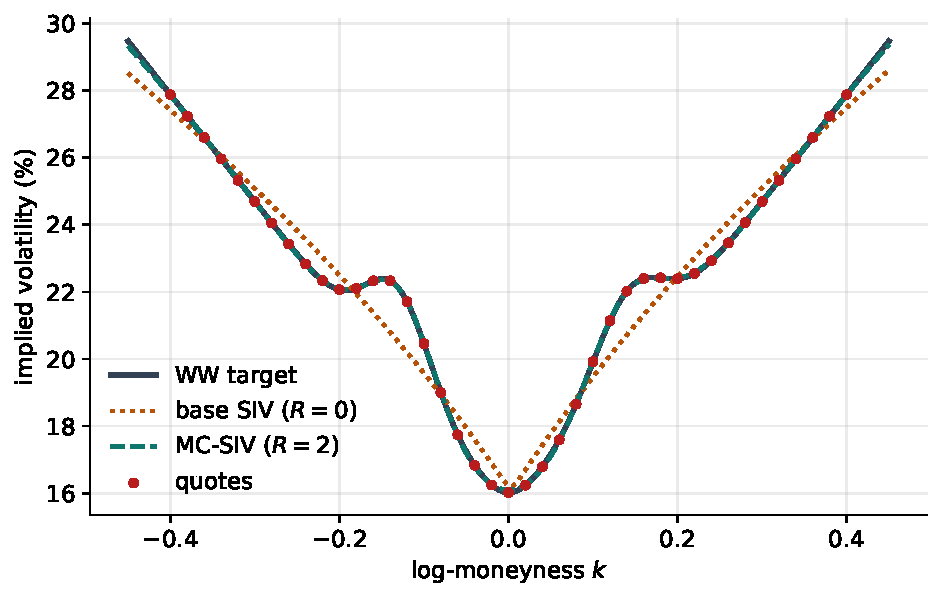
\includegraphics[width=0.80\textwidth]{fig_siv_fit.pdf}
\caption{The WW smile: the convex base ($R=0$, dotted) misses the shoulders by
\sivbasemaxerr\ vol bps; the two-core MCS fit (dashed) reaches \sivmaxerr\ vol
bps.}
\label{fig:fit}
\end{figure}

\begin{figure}[H]
\centering
\begin{minipage}{0.52\textwidth}\centering
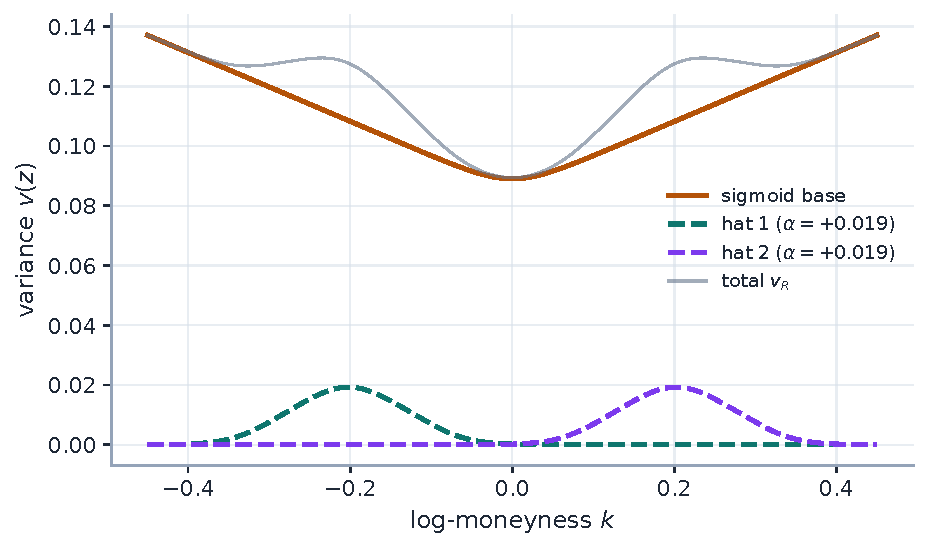
\includegraphics[width=\textwidth]{fig_siv_components.pdf}\\[1pt]
{\footnotesize (a) base $+$ two signed hats}
\end{minipage}\hfill
\begin{minipage}{0.45\textwidth}\centering
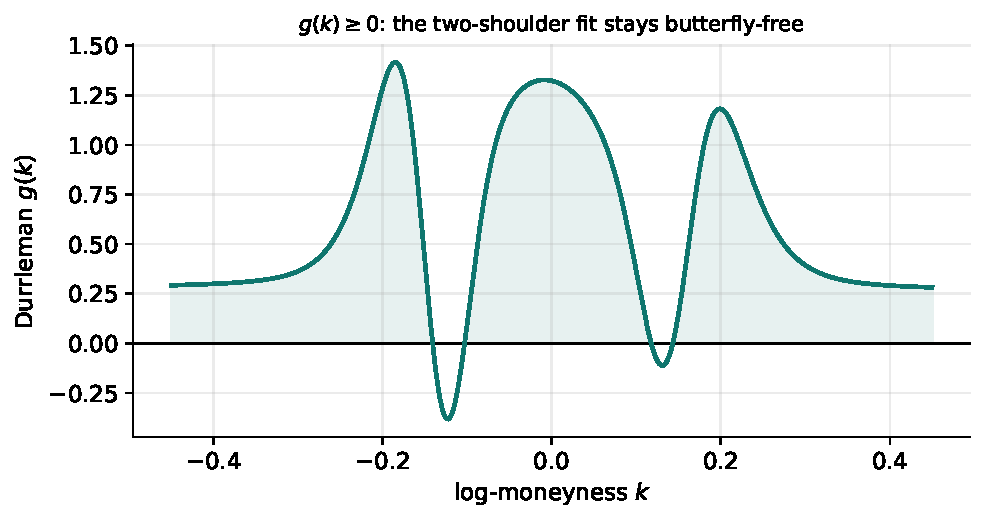
\includegraphics[width=\textwidth]{fig_siv_g.pdf}\\[1pt]
{\footnotesize (b) Durrleman $g(k)\geq0$, fit and target}
\end{minipage}
\caption{Left: the additive decomposition --- the convex base owns the wings, the
hats own the shoulders. Right: the butterfly diagnostic for both curves ---
the fitted slice and the synthetic target it chased --- non-negative on the
display window and, by the wide-grid assertion plus the analytic tail limits,
globally.}
\label{fig:components}
\end{figure}

\begin{remark}[The target must be clean too --- a bug fixed twice]
\label{rem:targetbug}
A diagnostic is only as strong as the exercise it certifies, and this
figure's target needed two rounds of honesty. An early revision built a WW
target whose \emph{own} Durrleman function dipped to $g\approx-0.38$ near the
shoulders: the synthetic ``market'' itself carried butterfly arbitrage, so no
admissible slice could both track it closely and honour $g\ge0$, and the
figure's claim was quietly false. The first fix re-chose the shoulder
amplitudes and widths (the shoulder-top curvature scales like $2A/s^2$ and is
what drives $w''$, hence $g$, negative) --- but that target was built in
\emph{volatility} space with $\sim0.20|k|$ tails, so its total variance grew
quadratically and still violated Lee far outside the plotted window: the
cleanliness was only per-window. The current construction builds the target
in \emph{total-variance} space --- hyperbolic base $+$ Gaussian shoulders ---
so the $w$-wings are exactly linear ($\beta=\sivtargetbeta\le2$) and the tail
$g$ limit $(4-\beta^2)/16$ is positive analytically; the generator computes
$g$ from analytic jets (no finite differences, the measurement lesson of
Note~02) and asserts $g>0$ for target \emph{and} fit on a dense grid to
$|k|=12$ before any figure is written. Current wide-grid values: target
$\min g=\sivtargetgmin$, fitted slice $\min g=\sivfitgmin$
(\nolinkurl{figures/gen_siv.py}; locked by
\nolinkurl{test_sigmoid.py::test_note03_ww_target_globally_clean}).
\end{remark}

%======================================================================
\section{Original ideas, and the over-fit caution}
\label{sec:original}

The genuinely original elements are the \emph{zero-wing hat}
\eqref{eq:hat}--\cref{lem:zerowing} --- a correction basis that is local in the
body and provably neutral in the wings, so expressiveness and tail control are
decoupled --- and the \emph{layered three-stage calibration} that places the hats
on residuals rather than optimizing them blind. Together they let one model span
from a clean index smile ($R=0$ --- the sigmoid base itself, a different
convex family from SVI, not an SVI equivalent) to an event-shaped WW smile
($R=2$) on a single slider. (A WW \emph{implied-volatility} curve suggests,
but does not by itself prove, a bimodal risk-neutral density --- the density
is the Breeden--Litzenberger second derivative of price, not a re-reading of
the vol curve.)

\begin{caution}
With great expressiveness comes over-fitting. The offline backtest (project
\texttt{backtest/}) found that on liquid index chains the Multi-Core hats
\emph{over-fit}: cores chase quote noise and manufacture butterfly-arbitrage
(the analytic diagnostic flags $g<0$ on a majority of calibrated nodes at $R\ge2$
on dense data), while the base $R=0$ behaves comparably to SVI; the extra
cores buy in-sample error and give most of it back out-of-sample. The honest
marginal number for the third core, from the spike replay: OOS RMS
$13.99\to13.58$ bp --- a $0.41$ bp improvement --- for roughly four times the
historical fit cost ($514\to2023$ ms in that harness) and worse arbitrage.
Not ``negative precision'', but nowhere near worth it. Two measures followed. The amplitude ridge,
the identifiability cap \eqref{eq:identifiability}, and the $g$ diagnostic mitigate
the fit itself; the surfaced slider is \emph{hard-capped at two} (\cref{sec:calib});
and the put-wing regularizer \eqref{eq:wingpen} of \cref{sec:wingpen} is default-on
to catch the residual wing violations that remain within the cap. The operational
guidance is unchanged: \emph{use cores only when the smile is genuinely non-convex}
(events, bimodal positioning), and prefer LQD or Local-Vol for routine fitting. The
cores slider is a scalpel, not a default.
\end{caution}

\begin{remark}[Two defences, one pathology --- and they are complementary]
The put-wing violation has \emph{two} sources: the flexible MCS genuinely
over-reaching (cured by \eqref{eq:wingpen}), and \emph{arbitraged inputs} --- the
per-strike de-Americanization of Note~05 can hand every model a call curve that is
already slightly non-convex in the wings. An ablation isolating the two defences
(the de-Am convex repair of Note~05 versus the penalty \eqref{eq:wingpen}) on
illiquid American ETFs found them \emph{complementary, not redundant}. On the
arb-prone population (medians over 38 nodes): with neither, worst-point
$g\approx-30$ and in-sample RMS $92$ bp; the de-Am repair alone cuts the
violation about threefold \emph{and lowers} the RMS to $25$ bp (it removes the
arbitraged quotes the model was chasing); the penalty alone nearly eliminates
the violation (median $\min g\ge-0.02$) but at $749$ bp (it must fight those
same quotes); both attain the penalty's arbitrage reduction at $225$ bp,
because the inputs are cleaned before the constraint is imposed. Reduction,
not elimination: even with both defences on, $26\%$ of the illiquid
population stays flagged --- neither defence \emph{guarantees} $g\ge0$. One
real node makes the mechanism vivid (EFA in the Aug-2024 vol spike, 11 days
to expiry, 22 quotes): neither defence, $75$ bp with worst $g=-116$; repair
alone, a tight $18$ bp but $g=-12$ remains; penalty alone, arbitrage-free but
$726$ bp; both, arbitrage-free at $34$ bp. The fence is expensive only when
it must fight arbitraged inputs --- the repair is what makes it affordable.
On liquid names the two defences behave differently, and only one is a no-op:
the de-Am \emph{repair} never fires there (dense chains have convex de-Am
wings --- byte-identical, confirmed on real data), but on the \emph{flagged}
liquid subset (17 of 30 audited nodes) the \emph{penalty} genuinely trades
fit for cleanliness: median in-sample error $10.9\to36.9$ bp with $41\%$
still flagged. That trade is the price of the fence where the violations are
shallow ($\min g\approx-0.23$) and the quotes dense. The quantitative case
for shipping both on by default stands on the illiquid population; the census
that sited the penalty (64\% put wing on the audited SIV-3 spike refits,
median worst violation at $z\approx-3.2$) and the cross-model framing are
Note~09's case file and confinement principle.
\end{remark}

%======================================================================
\section{Traceability}
\label{sec:traceability}

A scoping word first: the ``zero-wing / diagnostics'' rows below anchor
Note 03's \emph{current} construction; the legacy three-core golden tests
(\texttt{test\_note\_table1\ldots} etc., from the superseded design note's
sharper synthetic) lock the library's uncapped $R=3$ behaviour and are kept as
regression tripwires, not as evidence for this note's figures --- the
regenerated two-core example now has its \emph{own} lock. The penalty rows
are locked with stated tolerances: penalty-off is byte-identical
(\texttt{assert\_array\_equal}); penalty-on over a clean slice is unchanged
to $10^{-9}$ relative; and the repair test accepts a repaired
$\min g\ge-0.05$, not exactly zero.

\begingroup
\small
\setlength{\tabcolsep}{4pt}
\renewcommand{\arraystretch}{1.15}
\begin{longtable}{@{}p{0.36\textwidth}p{0.10\textwidth}p{0.50\textwidth}@{}}
\caption{Claims in this note and the code/tests that lock them.}\\
\toprule Claim & Object & Code anchor \newline \emph{Test anchors}\\ \midrule
\endfirsthead
\toprule Claim & Object & Code anchor \newline \emph{Test anchors}\\ \midrule
\endhead
Hat is unit-height, flat at centre, zero-wing in value/slope/curvature &
\cref{lem:zerowing} &
\nolinkurl{models/sigmoid/kernels.py}\newline
\nolinkurl{test_sigmoid.py::test_hat_is_zero_wing_and_unit_height}\\
\addlinespace
Wing slopes preserved under cores; $g$ and $\min v$ diagnostics match note &
\eqref{eq:wing_slopes} &
\nolinkurl{models/sigmoid/sigmoid.py}\newline
\nolinkurl{test_sigmoid.py::test_note_arbitrage_diagnostics}\\
\addlinespace
Reported $g$ is the priced (floored) curve's functional; degenerate slices
flagged not-free &
\cref{sec:noarb} &
\nolinkurl{models/sigmoid/sigmoid.py::gatheral_g}\newline
\nolinkurl{test_sigmoid.py::test_floored_diagnostic_is_priced_curve_functional}\\
\addlinespace
This note's two-core WW example (fit tight, base misses shoulders; target
and fit globally butterfly-clean) &
\cref{sec:example} &
\nolinkurl{models/sigmoid/calibrate.py}\newline
\nolinkurl{test_sigmoid.py::test_note03_ww_two_core_example_regression}\newline
\nolinkurl{::test_note03_ww_target_globally_clean}\\
\addlinespace
Cores improve the WW fit monotonically (legacy synthetic) &
\cref{sec:example} &
\nolinkurl{models/sigmoid/calibrate.py}\newline
\nolinkurl{test_sigmoid.py::test_more_cores_fit_better_on_ww_smile}\\
\addlinespace
Hat-count cap $R\le\lfloor(N-6)/4\rfloor$ (hats only; the base still fits at
$N=5$) &
\eqref{eq:identifiability} &
\nolinkurl{models/sigmoid/calibrate.py}\newline
\nolinkurl{test_sigmoid.py::test_cores_are_capped_to_quote_count}\\
\addlinespace
Surfaced slider clamped to two (schema boundary, every parse) &
\cref{sec:calib} &
\nolinkurl{api/schemas.py}\newline
\nolinkurl{test_siv_wing_penalty.py::test_cores_clamped_to_two}\\
\addlinespace
Put-wing hinge repairs wing arb (to $\min g\ge-0.05$); clean slices unchanged
($10^{-9}$ rel); off by library default (byte-identical) &
\eqref{eq:wingpen} &
\nolinkurl{models/sigmoid/calibrate.py}\newline
\nolinkurl{test_siv_wing_penalty.py::test_penalty_removes_wing_arb}\newline
\nolinkurl{::test_penalty_byte_identical_on_arb_free_slice}\newline
\nolinkurl{::test_penalty_off_default}\\
\addlinespace
Analytic Jacobian matches FD (base, cores, band, calendar) &
\cref{sec:calib} &
\nolinkurl{models/sigmoid/jacobian.py}\newline
\nolinkurl{test_sigmoid_jacobian.py::test_two_cores_mid}\newline
\nolinkurl{::test_two_cores_band}\newline
\nolinkurl{::test_calendar_active}\\
\addlinespace
Curve identified, parameters deliberately not &
\cref{sec:calib} &
\nolinkurl{models/sigmoid/calibrate.py}\newline
\nolinkurl{test_sigmoid.py::test_round_trip_curve_recovery}\\
\addlinespace
Prior blocks reach the MCS overlay &
\cref{sec:calib} &
\nolinkurl{models/sigmoid/calibrate.py}\newline
\nolinkurl{test_prior_parametric.py::test_operator_prior_pulls_all_models_toward_prior_skew}\\
\addlinespace
R3$\times$R6 ablation numbers &
\cref{sec:original} &
\nolinkurl{backend/backtest/ablation_arb.py}\newline
\nolinkurl{test_ablation_arb.py}\\
\addlinespace
WW figure target and fit butterfly-clean globally (dense grid to $|k|=12$
$+$ analytic tail limits) &
\cref{rem:targetbug} &
\nolinkurl{figures/gen_siv.py}\newline
runtime assertions in the generator $+$ the two example tests above\\
\bottomrule
\end{longtable}
\endgroup

\appendix
%======================================================================
\section{Hyperparameter atlas}
\label{app:atlas}

\begin{longtable}{p{0.24\textwidth}p{0.14\textwidth}p{0.54\textwidth}}
\caption{Multi-Core Sigmoid (MCS) hyperparameters.}\label{tab:atlas}\\
\toprule Knob & Default & Role\\ \midrule
\endfirsthead
\toprule Knob & Default & Role\\ \midrule
\endhead
\multicolumn{3}{@{}p{0.95\textwidth}@{}}{\emph{Surfaced. Product defaults
shown (the product's default model is LQD; these apply when MCS is
selected). Library defaults differ: $R=0$, penalty off.}}\\ \midrule
\texttt{nCores} $R$ (\texttt{FitSettings}) & $2$ & Number of zero-wing hats,
$R\in\{0,1,2\}$ (schema-clamped at two on \emph{every} parse --- persisted or
fresh; the library itself is uncapped, and the identifiability bound
\eqref{eq:identifiability} may reduce $R$ further). $0$ = pure sigmoid base.\\
\texttt{sivWingPenaltyPct} $\Lambda$ (\texttt{OptionsSettings}) & $100$ &
Put-wing Durrleman penalty \eqref{eq:wingpen} strength; $100=$ base
$\lambda_0=10^{3}$, $0=$ off.\\
\texttt{sigmoidRidge} $\varrho$ (\texttt{FitSettings}) & \sivridge & $\ell^2$
penalty on hat amplitudes in the refine stage.\\
\texttt{midAnchorWeight} & $0.05$ & Band-fit mid anchor (Note~07).\\
\texttt{weightScheme} & \texttt{equal} & Per-quote weights (Note~07).\\
\texttt{calendarWeight} & $10^{6}$ & Calendar hinge penalty (Note~10;
\texttt{OptionsSettings}).\\
\texttt{extrapEnforce} & off & Tapered extrapolated-region fences (Notes
09--10; \texttt{OptionsSettings}); hybrid Jacobian when on.\\
\midrule
\multicolumn{3}{l}{\emph{Internal (seeding / bounds)}}\\ \midrule
\texttt{\_H\_INIT} & \sivhinit & Hat half-width seed.\\
\texttt{\_KAPPA\_INIT} & \sivkappainit & Hat steepness seed.\\
\texttt{\_H\_BOUNDS} & $[\sivhlo,\sivhhi]$ & Hat half-width bounds.\\
\texttt{\_KAPPA\_BOUNDS} & $[\sivkappalo,\sivkappahi]$ & Hat steepness bounds.\\
\texttt{\_C\_PAD} & $0.5$ & Centre padding beyond the quoted $z$-range.\\
\texttt{\_V\_FLOOR} & $10^{-8}$ & Variance floor so $\sqrt v$ stays real.\\
\texttt{\_LOGCOSH\_CLIP} & $50$ & $|x|$ beyond which $\log\cosh$ uses its asymptote.\\
\texttt{xtol/ftol} & $10^{-12}$ & trf tolerances.\\
\bottomrule
\end{longtable}

%======================================================================
\section{Performance notes}
\label{app:perf}

\begin{enumerate}[leftmargin=1.6em]
\item \textbf{Analytic Jacobian} through the log-cosh primitive replaces the
$(6+4R+1)$-evaluation finite difference; measured \sivspeedup$\times$ on the
\emph{final-refine microbenchmark} (the $R=2$ mid refine alone --- base fit,
seeding and the product-default wing penalty excluded; single-threaded
development machine, fastest of three), optimum unchanged to $\sivcostdiff$.
Gated to the var-swap/prior-free path. When the put-wing penalty
\eqref{eq:wingpen} or \texttt{extrapEnforce} is active, only the small penalty
grids are finite-differenced (a \emph{hybrid} Jacobian), so the penalized fit
retains most of this speed.
\item \textbf{Layered warm start.} Fitting the base first and seeding hats on its
residual gives the joint refine an excellent start, so the bounded trf converges
quickly even with several cores.
\item \textbf{Vectorized kernels.} $\Phi,\Phi',\Phi''$ and the hat second
differences are NumPy-vectorized and side-effect free, shared between the model
and its Jacobian.
\item \textbf{Identifiability cap.} Limiting $R$ by the quote count avoids wasting
iterations on under-determined narrow kernels and is the first line of defence
against the over-fit of \cref{sec:original}.
\end{enumerate}

%======================================================================
\section{Reference implementation}
\label{app:ref}

Building on \cref{lst:hat}, the full slice $v_R(z)$ \eqref{eq:model} and the
butterfly diagnostic $g(k)$ \eqref{eq:durrleman_siv} are a few more lines. The
$z$-jets (value, slope, curvature) are carried together because $g$ needs all
three; \texttt{\_dhat} forms a hat or either of its derivatives from the matching
$\Phi$-jet, so the zero-wing second difference is written once. Verified against
\texttt{MultiCoreSiv} on a two-core benchmark to $10^{-13}$.

\begin{lstlisting}[caption={The full model $v_R(z)$ and Durrleman $g(k)$
(distilled from \texttt{models/sigmoid/\{kernels,sigmoid\}.py}).}]
def phi_p(u, k):  return (2/k) * np.tanh(k*u/2)        # Phi'
def phi_pp(u, k): return 1 / np.cosh(k*u/2)**2         # Phi''
def _dhat(f, z, c, h, kappa):                          # B or a B-derivative
    u = z - c                                          #   from the matching Phi-jet
    return (f(u-h,kappa) - 2*f(u,kappa) + f(u+h,kappa)) / (2*phi(h, kappa))

def v_model(z, base, cores):
    """MCS variance v_R(z) = v_base(z) + sum_r alpha_r B_r(z), with z-jets."""
    v0, s0, k0, z0, kp, kc = base
    u = z - z0
    kappa = np.where(u < 0, kp, kc)                    # asymmetric wings, C^2 at z0
    v, vz, vzz = v0 + s0*u + k0*phi(u,kappa), s0 + k0*phi_p(u,kappa), k0*phi_pp(u,kappa)
    for alpha, c, h, kap in cores:                     # add the signed zero-wing hats
        v   += alpha * _dhat(phi,    z, c, h, kap)
        vz  += alpha * _dhat(phi_p,  z, c, h, kap)
        vzz += alpha * _dhat(phi_pp, z, c, h, kap)
    return v, vz, vzz

def durrleman_g(z, base, cores, t, sigma_ref):
    """Butterfly diagnostic g(k) >= 0; converts z-space jets to k-space."""
    v, vz, vzz = v_model(z, base, cores)
    k, w = sigma_ref*np.sqrt(t)*z, t*v
    wk, wkk = np.sqrt(t)/sigma_ref*vz, vzz/sigma_ref**2
    return (1 - k*wk/(2*w))**2 - 0.25*wk**2*(1/w + 0.25) + 0.5*wkk
\end{lstlisting}

\begin{thebibliography}{9}
\bibitem{Gatheral2006} J.~Gatheral. \emph{The Volatility Surface: A Practitioner's
Guide}. Wiley, 2006.
\bibitem{Durrleman2010} V.~Durrleman. From implied to spot volatilities.
\emph{Finance and Stochastics}, 14(2):157--177, 2010.
\bibitem{Lee2004} R.~W.~Lee. The moment formula for implied volatility at extreme
strikes. \emph{Mathematical Finance}, 14(3):469--480, 2004.
\end{thebibliography}

\end{document}
